\documentclass[10pt]{extarticle}

\usepackage{preamble_base}
\usepackage{preamble_math}

\usepackage{siunitx}
\usepackage{esint} % for closed integrals

\title{Physics Exercises}
\date{Semester 2, 2023/2024}

\setlength{\headheight}{15pt} % ??? we do what fancyhdr tells us to do

% Units
\DeclareSIUnit\angstrom{Å} % Redefine it as it got deprecated
\DeclareSIUnit\atm{atm}
\DeclareSIUnit{\calorie}{cal}

\newcommand{\anglebraces}[1]{
    \langle #1 \rangle
}

\newcommand{\horizonalline}{\noindent\rule{\textwidth}{1pt}}

\tcbuselibrary{theorems}
\newtcbtheorem[number within = subsection]{question}{Question}{
    parbox = false, % for parskip
    breakable,
    % stuff for the border
    enhanced,
    sharp corners,
    boxrule = 0pt,
    frame hidden,
    borderline west = {0.25em}{1pt}{orange},
    % title
    detach title,
    before upper = {\tcbtitle\enspace},
    description delimiters parenthesis,
    description font = \mdseries,
    terminator sign = {.},
    separator sign none,
    fonttitle = \bfseries,
    % colors
    coltitle = orange,
    colback = orange!10!white,
}{qs}

\newtcolorbox{solution}{
    parbox = false, % for parskip
    breakable,
    % stuff for the border
    enhanced,
    sharp corners,
    boxrule = 0pt,
    frame hidden,
    borderline west = {0.25em}{1pt}{blue},
    % title
    title = {Solution.},
    detach title,
    before upper = {\tcbtitle\enspace},
    fonttitle = \itshape,
    % colors
    coltitle = blue,
    colback = blue!10!white,
}


\begin{document}

\firstpage

\section{24 Jan 2024}

\subsection{First partial}

\begin{question}{}{jan_24_2}
    Astronaut with mass $M$ at $v_0$. Ejects $m_g$ at $v_g$.
    \begin{enumerate}
        \item Find $v_g$ s.t. $v' = 0$
        \item Eject $m_g$ 3 times: find final $v$
        \item Total gas is $20m_g$. Find $v_0$ s.t. cannot invert direction
    \end{enumerate}
\end{question}

\begin{solution}
    We use conservation of momentum.
    \begin{enumerate}
        \item Since we need $v' = 0$:
              \begin{equation}
                  Mv_0 = m_g (\cancel{v'} + v_g) + \cancel{(M - m_g) v'} \implies v_g = v_0\frac{M}{m_g}
              \end{equation}
        \item Repeat the argument
              \begin{align}
                  Mv_0 & = m_g (v' + v_g) + (M - m_g) v'                                        \\
                       & =  m_g (v' + v_g) + m_g(v'' + v_g) + (M - 2m_g) v''                    \\
                       & =  m_g (v' + v_g) + m_g(v'' + v_g) + m_g(v''' + v_g) + (M - 3m_g) v'''
              \end{align}

              Now solve for each $v$: for $v'$ we have
              \begin{multline}
                  Mv_0 = \cancel{m_g v'} + m_g v_g + M v' - \cancel{m_g v'} \\
                  \implies v' = \frac{Mv_0 - m_g v_g}{M}
              \end{multline}
              for $v''$
              \begin{multline}
                  \cancel{m_g v'} + m_g v_g + M v' - \cancel{m_g v'} =  m_g v' + 2m_g v_g - m_g v'' + M v'' \\
                  \implies v'' = \frac{v'(M - m_g) - m_g v_g}{ M - m_g} = v' - \frac{m_g v_g}{M - m_g}
              \end{multline}
              and for $v'''$
              \begin{multline}
                  \cancel{m_g v'} + 2m_g v_g + \cancel{m_g v''} + M v'' - 2m_g v'' = \cancel{m_g v'} + 3m_g v_g + \cancel{m_g v''} + M v''' - 2m_g v''' \\
                  \implies v''' = \frac{(M -2m_g)v'' - m_g v_g}{M - 2m_g} = v'' - \frac{m_g v_g}{M - 2m_g}
              \end{multline}
        \item We noted how some velocity $v^{(n)}$ can be written as
              \begin{equation}
                  v^{(n)} = v_0 - \sum_{k = 0}^{n-1} \frac{m_g v_g}{M - k m_g}
              \end{equation}
              then we need $v^{(20)} > 0$ so
              \begin{equation}
                  \sum_{k = 0}^{19} \frac{m_g v_g}{M - k m_g} < v_0
              \end{equation}
    \end{enumerate}
\end{solution}

\subsection{Second partial}

\begin{question}{}{}
    A sphere and a cylinder are released on an inclined plane, starting stationary and from the same height.
    The two objects have the same mass and radius.
    In the condition of pure rolling, who arrives down first? Who arrives first if there is no friction instead?
\end{question}

\begin{solution}
    Consider the moment of inertia of the two objects:
    \begin{align*}
        I_\text{sphere}   & = \frac{2}{5} m r^2 \\
        I_\text{cylinder} & = \frac{1}{2}mr^2
    \end{align*}

    Then we can apply conservation of energy as follows:
    \begin{equation}
        mgh = \half mv_{cm} + \half I \omega
    \end{equation}
    where the only changing part between the two is the moment of inertia.

    Since $I_\text{sphere} < I_\text{cylinder}$ the cylinder's speed will be less than the one of the sphere at every time, therefore the sphere arrives first.

    If there is no friction, then there is no rolling and the two energy equations are equivalent and they arrive at the same time.
\end{solution}

\noindent\rule{\textwidth}{1pt}

\begin{question}{Exercise 1}{24_jan_24_p2_ex_1}
    Disks of $M_1, M_2$ and $R_1, R_2$ with $R_1 > R_2$. Point masses $m_1, m_2$ on frictionless planes inclined $\theta$.
    Two ropes $m_1$ to $R_1$, $m_2$ to $R_2$. No slipping.

    \begin{enumerate}
        \item Find $\alpha$ of the pulley
        \item At $t=0$ masses at same height at rest. At $t^*$ $m_1$ has risen by $h_1$. Find $\omega$
        \item Find $\mu_s$ for $m_2$ s.t. equilibrium
    \end{enumerate}
\end{question}

\begin{solution}
    Consider $\hat z$ the direction going into the diagram.

    \begin{enumerate}
        \item \label{itm:24_jan_24_p2_ex_1:1} We just use $\tau = I \alpha$ and $F = ma$ where $I = \half M_1 R_1^2 + \half M_2 R_2^2$.
              \begin{align}
                  \begin{cases}
                      T_2 R_2 - T_1 R_1 = \left(\half M_1 R_1^2 + \half M_2 R_2^2 \right) \alpha \\
                      T_1 - m_1 g \sin \theta = m_1 \alpha R_1                                   \\
                      m_2 g \sin \theta - T_2 = m_2 \alpha R_2                                   \\
                  \end{cases}
              \end{align}

              Substituting we get
              \begin{gather}
                  (m_2 g \sin \theta - m_2 \alpha R_2) R_2 - (m_1 g \sin \theta + m_1 \alpha R_1) R_1 = \left(\half M_1 R_1^2 + \half M_2 R_2^2 \right) \alpha\\
                  2m_2 g \sin \theta R_2 - 2m_2 \alpha R_2^2 - 2m_1 g \sin \theta R_1 + 2m_1 \alpha R_1^2 = (M_1 R_1^2 + M_2 R_2^2) \alpha \\
                  2g \sin \theta (m_2 R_2 - m_1 R_1) = (M_1 R_1^2 + M_2 R_2^2 + 2m_2 R_2^2 - 2m_1 R_1^2) \alpha \\
                  \alpha = 2g \sin \theta \frac{m_2 R_2 - m_1 R_1}{M_1 R_1^2 + M_2 R_2^2 + 2m_2 R_2^2 - 2m_1 R_1^2}
              \end{gather}

              $\implies \alpha = 2g \sin \theta \frac{m_2 R_2 - m_1 R_1}{M_1 R_1 + M_2 R_2}$

        \item Use conservation of energy.
              Set zero gravitational potential is height at rest, then the initial energy is $0$.
              \begin{equation}
                  0 = m_1 g h_1 - m_2 g h_2 + \half \left( \half M_1 R_1^2 + \half M_2 R_2^2 \right) \omega^2 + \half m_1 v_1^2 + \half m_2 v_2^2
              \end{equation}

              We now need to express the following values w.r.t. known ones:
              \begin{itemize}
                  \item We know that $\frac{h_1}{\sin \theta} \frac{1}{2 \pi R_1} = \frac{h_2}{\sin \theta}\frac{1}{2 \pi R_2}$ and simplifying we get
                        $h_2 = h_1 \frac{R_2}{R_1}$.
                  \item The two velocities can be expressed as $v_i = \omega R_i$.
              \end{itemize}
              then we can write the equation as
              \begin{gather}
                  0 = m_1 g h_1 - m_2 g h_1 \frac{R_2}{R_1} + \half \left( \half M_1 R_1^2 + \half M_2 R_2^2 \right) \omega^2 + \half m_1 (\omega R_1)^2 + \half m_2 (\omega R_2)^2 \\
                  gh_1 \left(m_2 \frac{R_2}{R_1} - m_1 \right) = \half \omega^2 \left( \half M_1 R_1^2 + \half M_2 R_2^2 + m_1 R_1^2 + m_2 R_2^2 \right) \\
                  \frac{4 g h_1}{R_1} (m_2 R_2 - m_1 R_2 ) = \omega^2 ( M_1 R_1^2 + M_2 R_2^2 + 2 m_1 R_1^2 + 2 m_2 R_2^2 ) \\
                  \omega = \sqrt{\frac{4 g h_1 (m_2 R_2 - m_1 R_2 )}{R_1 ( M_1 R_1^2 + M_2 R_2^2 + 2 m_1 R_1^2 + 2 m_2 R_2^2 )}}
              \end{gather}

        \item We use the same equations as in \ref{itm:24_jan_24_p2_ex_1:1} imposing equilibrium:
              \begin{align}
                  \begin{cases}
                      T_2 R_2 - T_1 R_1 = 0       \\
                      T_1 - m_1 g \sin \theta = 0 \\
                      m_2 g \sin \theta - T_2 - \mu_s m_2 g \cos \theta = 0
                  \end{cases}
              \end{align}

              Substituting we get
              \begin{gather}
                  m_2 \cancel{g} \sin \theta - m_1 \cancel{g} \sin \theta \frac{R_1}{R_2} - \mu_s m_2 \cancel{g} \cos \theta = 0 \\
                  \mu_s = \frac{m_2 \sin \theta R_2 - m_1 \sin \theta R_1}{m_2 \cos \theta R_2}
              \end{gather}
    \end{enumerate}
\end{solution}

\noindent\rule{\textwidth}{1pt}

\begin{question}{Exercise 2}{24_jan_24_p2_ex_2}
    Pipe with $L, A$ filled with helium at $p_\text{atm}$ in a lake of depth $d$ until water at $2L/3$ inside the pipe.
    $T$ lake constant.

    \begin{enumerate}
        \item Find $p$ the pressure of the helium inside the pipe. $\rho_{\text{He}} < \rho_w$.
        \item Depth $h$ of lower end of the pipe
        \item Hole at $h_1 < 2L/3$, find $v$.
    \end{enumerate}
\end{question}

\begin{solution}
    \begin{enumerate}
        \item Assume the helium gets compressed isothermally. Then
              \begin{equation}
                  p_\text{atm} L A = p \frac{L}{3} A \implies p = 3 p_\text{atm}
              \end{equation}

        \item We can use Stevino's law we get
              \begin{align}
                  p & = p_\text{atm} + \rho_w g \left(\frac{2}{3}L - h\right)            \\
                  h & = \frac{3p_\text{atm} + 2\rho_w g L - 3(3p_\text{atm})}{3\rho_w g} \\
                    & = \frac{2\rho_w g L - 6p_\text{atm}}{3\rho_w g}                    \\
                    & = \frac{2}{3}L - \frac{2 p_\text{atm}}{\rho_w g}
              \end{align}

        \item Use Bernoulli's law and, since the hole is very small, the velocity of the water in contact with the helium is negligible
              \begin{equation}
                  p + \rho_w g \left(d + \frac{2}{3}L + h\right) = p_\text{atm} + \rho_w g ( d - h + h_1) + \half \rho_w v^2
              \end{equation}
    \end{enumerate}
\end{solution}

\clearpage

\section{25 May 2024}
\subsection{First partial}

\begin{question}{}{}
    Explain the Michelson and Morley experiment.
\end{question}

\horizonalline

\begin{question}{}{}
    Let $\vec F(x, y, z) = \left(x(1-x^2), 3+y^3, f_z(x, y, z)\right)$. Find $f_z(x, y, z)$ s.t. $\vec F$ conservative.
\end{question}

\horizonalline

\begin{question}{}{}
    $m_1, m_2$, massless pulleys. The higher pulley cannot move, the lower can.

    \emph{Tip:} massless bodies mus receive zero net force or this would cause infinite acceleration.

    \begin{enumerate}
        \item Spring constant $\kappa$, $2m_2 > m_1$, find $\Delta l$ in equilibrium.
        \item Cut the string between spring and $m_1$, find $a$ of $m_2$.
    \end{enumerate}

    \begin{figure}[H]
        \centering
        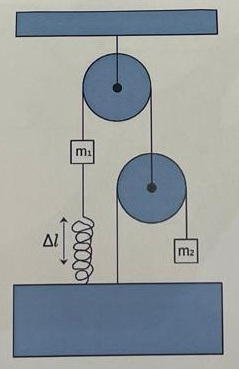
\includegraphics[width=0.25\textwidth]{assets/S2_P2_PHY1_Exercises/25_may_24-ex1.jpg}
        \caption{Problem's setup}
    \end{figure}
\end{question}

\horizonalline

\begin{question}{}{}
    Projectile $m$ at angle $\theta$ shot with kinetic energy $K_0$.
    When $K = U$ the projectile explodes in two halves of $m/2$.

    \begin{enumerate}
        \item Find the minimum $\theta$ s.t. the explosion can happen
        \item Given $\theta$ from above, one fragment goes back where it started. Where does the other one land?
    \end{enumerate}
\end{question}

\subsection{Second partial}

\begin{question}{}{}
    Is a rotation necessary to have a non-zero angular momentum? Provide an example.
\end{question}

\horizonalline

\begin{question}{}{}
    Why is there an upper limit for the efficiency $\eta < 1$ of a thermal engine working between $T_H$ and $T_C$?
    What is this limit?
\end{question}

\horizonalline

\begin{question}{}{}
    Spool of mass $M$, $R, r$ and $I$. Constant force $F$, the spool moves in the direction of $F$.

    \begin{enumerate}
        \item $a_{cm}$ of spool.
        \item $F$ is given by a mass $m$ with massless pulley. From equilibrium, find velocity of $m$ at $h$.
    \end{enumerate}

    \begin{figure}[H]
        \centering
        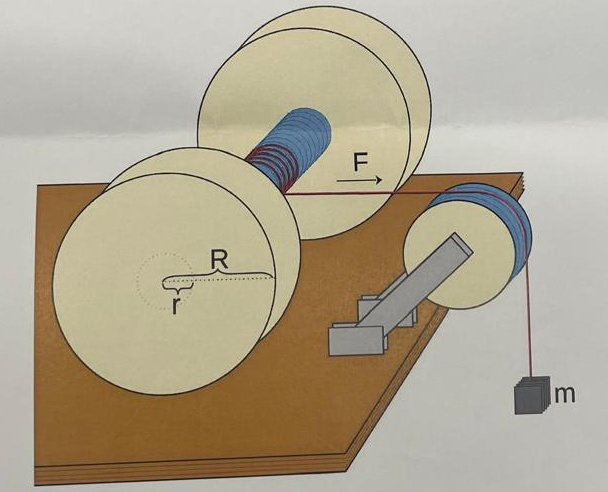
\includegraphics[width=0.35\textwidth]{assets/S2_P2_PHY1_Exercises/25_may_24-ex2.jpg}
        \caption{Problem's setup}
    \end{figure}
\end{question}

\horizonalline

\begin{question}{}{}
    A container with large $A$ holds two liquids of densities $d$ and $2d$ each of $H/2$. The top liquid has $p_\text{atm}$.
    A cylinder of length $L < H/2$ and area $A/5$ is immersed s.t. it floats vertically with $L/4$ in the dense liquid.

    \begin{enumerate}
        \item Find $\rho$ of the cylinder.
        \item Find total pressure at the bottom of the container.
        \item Initially cylinder fixed at $H/2 - L/4 + x$, at $t = 0$ starts oscillating. Initial displacement from equilibrium $x$ is small.
              Compute the frequency of the vertical oscillation.
    \end{enumerate}

    \begin{figure}[H]
        \centering
        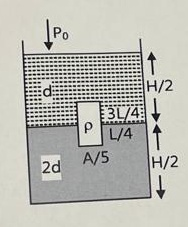
\includegraphics[width=0.25\textwidth]{assets/S2_P2_PHY1_Exercises/25_may_24-ex3.jpg}
        \caption{Problem's setup}
    \end{figure}
\end{question}

\end{document}
